%
% File eamt11.tex, adapted from eamt10.tex
%
% Contact: vincent@ccl.kuleuven.be

%%% To ease future customizations, various replaceables have been paramaterized
%%% as listed in the newcommands section

\documentclass[11pt]{article}
\usepackage[utf8x]{inputenc}
\usepackage{eamt11}
\usepackage{url}
\usepackage{times}
\usepackage{multirow}
\usepackage[small,bf]{caption}
\usepackage{latexsym}
\usepackage{graphicx}
\usepackage{gb4e}
\usepackage{linguex} %think it has to be the last package

\setlength\titlebox{6.5cm}    % Expanding the titlebox

\newcommand{\confname}{EAMT 2011}
\newcommand{\website}{http://www.eamt2011.eu/}
\newcommand{\contactname}{the programme chairs Mikel Forcada \& Heidi De Praetere}
\newcommand{\contactemail}{mlf@dlsi.ua.es} 
\newcommand{\conffilename}{eamt11}
\newcommand{\downloadsite}{http://www.eamt2011.eu/}
\newcommand{\paperlength}{$8$ (eight)}
\newcommand{\shortpaperlength}{$4$ (four)}

\title{Rapid rule-based machine translation between Dutch and Afrikaans}

\author{Pim Otte\\
  Mendelcollege\\
  Pim Mulierlaan 4\\
  2024 BT Haarlem\\
  {\tt 5666@mendelcollege.nl}  \And
  Francis M. Tyers\\
  Dept. Lleng. i Sist. Inform.\\
  Universitat d'Alacant\\
  E-03070 Alacant \\
  {\tt ftyers@dlsi.ua.es}}

\date{}

\begin{document}
\maketitle
\begin{abstract}
 This paper describes the design, development and evaluation of a machine
 translation system between Dutch and Afrikaans developed over a period of
 around a month.
\end{abstract}

\section{Introduction}

The Dutch language is West-Germanic and is spoken by nearly 23 million people, which are 
mostly from the Netherlands and Flanders, the Dutch-speaking part of Belgium and a minority 
live in former colonies of the Netherlands, such as Suriname, Aruba and the Netherlands 
Antilles. The Dutch language as it is today, started developing in the 16th century in the 
major trade cities, such as Amsterdam and Antwerp \cite{Shetter:02}.  Afrikaans is spoken 
by at least 5 million people, mainly in South Africa but also in Namibia. Afrikaans is a 
variety of Dutch that originates from the Dutch that was spoken by the Dutch colonists of 
the Cape Colony. In 1925 Afrikaans replaced Dutch as an official language in South Africa, to 
be the joint official language together with English. Currently Afrikaans is one of the 
eleven national languages \cite{Donaldson:93}.

In this paper we will describe the development of {\small {\tt apertium-af-nl}}, an Afrikaans 
and Dutch machine-translation system based on the Apertium platform. Since Afrikaans and Dutch 
are largely mutually intelligible, this machine translation system focuses on dissemination, the 
production of text for the purpose of being post-edited and then being published. Previous 
work in Afrikaans and Dutch machine translation is described in \cite{Huyssteen:09}. The reason
we have chosen to work with a rule-based approach, instead of the ubiquitous statistic approach,
is that the latter needs high-quality parallel corpora of both languages. The only freely available
Afrikaans Dutch corpus, is KDE4 \frootnote{\url{http://opus.lingfil.uu.se/KDE4v2.php}}. We feel
that these corpora do not approach the quality neccisated and the fact that Afrikaans and Dutch
are closely related languages made a rule-based approach favourable to the statistical approach.

The paper is laid out as follows, firstly, we will describe the reuse and creations of 
resources. We will then discuss several grammatical features of Afrikaans and Dutch and how 
these were incorporated in the machine-translation system. We will then present a section 
in which the system is evaluated. Finally, we will discuss the system and future work that 
could be done.


\begin{itemize}
\item languages, machine translation, existing work
\item rationale: no free corpora of dutch--afrikaans.
\end{itemize}

\section{Method}

The system is based on the Apertium machine translation platform.\footnote{\url{http://www.apertium.org}} The
platform was originally aimed at the Romance languages of the Iberian
peninsula, but has also been adapted for other, more distantly related,
language pairs. The whole platform, both programs and data, are licensed
under the Free Software Foundation's General Public
Licence\footnote{\url{http://www.fsf.org/licensing/licenses/gpl.html}} (GPL)
and all the software and data for the 25 supported language pairs (and the
other pairs being worked on) is available for download from the project
website.

\begin{figure*}
  \centering
  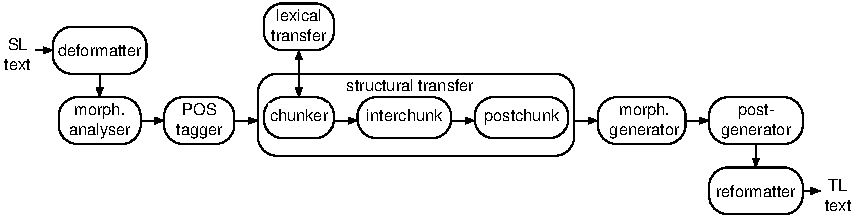
\includegraphics[scale=0.8]{apertium2.pdf}
  \caption{Modular architecture of the Apertium MT
    platform. The compound analysis and generation modules are included at the morphological
    analyser and morphological generator stages respectively.}
\label{fg:apertium}
\end{figure*}

{\small {\tt apertium-af-nl}} has been developed over the course of one and a half months.
The vast majority of the work has been done by a PhD student and a Dutch secondary 
school student. However, since for both this was not paid, nor for school, there were 
very few full 8-hour days of work during this period.

\begin{itemize}
\item development time, how apertium works (fig. 1)
\end{itemize}

\subsection{Existing resources}

One existing resource was reused with very little modification, that is the 
morphological transducer for Afrikaans created during a separate project on English--Afrikaans
machine translation. Some changes were made. The structure of verb entries
was wholly revised, and infrequent words were removed.

\subsection{Resources created}

\subsubsection{Dutch morphological transducer}

There are a number of existing morphological analysers for Dutch, based on ...

We chose to create a new analyser because... (tagset, gender, analysis/generation, free software)

The open categories (nouns, verbs, adjectives, adverbs) for the Dutch 
morphological analyser were extracted semi-automatically from 
Wiktionary,\footnote{\url{http://www.wiktionary.org}} a free online 
dictionary that often includes inflectional information. In the case 
of Dutch nouns it often (although not always) gives the gender and the 
plural and diminutive forms (see for example Figure~\ref{fig:wikt1}).
The category {\small {\tt Dutch nouns}} has a total of 10,610 entries,
while the corresponding category on the Dutch Wiktionary has 13,176 entries.

Closed categories were added by hand based on a grammar of Dutch \cite{Shetter:02}.

\begin{figure*}
\centering
\begin{small}
\begin{tabular}{|l|}
\hline
{\large Dutch} \\
~\\
{\bf Etymology}\\
~\\
~{\em hoofd-} (``main, head'') + {\em stad} (``city'')\\
~\\
{\bf Pronunciation}\\
~\\
{\bf Noun}\\
~\\
{\bf hoofdstad} m. ({\em plural} hoofdsteden, {\em diminutive} hoofdstadje, {\em diminutive} plural hoofdstadjes) \\
~\\
~~~~1. capital city \\

\hline
\end{tabular}
\end{small}
\caption{English language Wiktionary article for Dutch \emph{hoofdstad} `capital city' 
    {\small \url{http://en.wiktionary.org/wiki/hoofdstad}}}
\label{fig:wikt1}
\end{figure*}

\subsubsection{Bilingual dictionary}

The bilingual dictionary has been developed in several ways. After the morphological 
analysers for both languages were large enough, exact matches from the dictionaries
were automatically added to the bilingual dictionary. Proper names were added in the
way that is described in \cite{Tyers:08}. After that cognates were added. There are several
small common spelling differences between the Afrikaans and Dutch languages. For example,
where the letter `y' in Afrikaans is used quite often, the Dutch languages uses `ij' in these words.
The bilingual dictionary was expanded further by categorising these spelling differences and
automatically adding translations to the bilingual dictionary if the spelling difference was the
only difference between the two words. Finally, some entries were done by hand.
This includes closed categories, but also words that frequently appeared in Wikipedia
which were not yet in the bilingual dictionary.

\begin{itemize}
\item wikipedia, wiktionary, cognates
\end{itemize}

\subsubsection{Transfer rules}

%%Dutch cannot use the present tense in past situations (not even in narrative style)

Several transfer rules used in {\small {\tt apertium-af-nl}}  are characteristic for the
Afrikaans and Dutch languages. We will discuss some of these transfer rules below.

Firstly, Afrikaans has no genitives. Instead, the word `se' is used to indicate possesion. 
Therefore, a transfer rule has been added to remove the `se' and instead make the preceding
noun a genetive.

%af:Die vrou se seun.
%nl:De vrouws zoon.
%gloss:DEF.ARTICLE woman.NOUN.GEN son.NOUN

Secondly, the verb `he' (to have) is the only verb used in Afrikaans as auxiliary
verb with a past participle. In Dutch the verbs `hebben' and `zijn' (to have, to be)
are both used, the latter mostly in cases of movement and a few exceptional cases, the
former in all others. To handle this, two transfer rules have been added, to handle the
patterns `have + past participle' and `have + nie + past participle + nie', which change the
verb to have into the verb to be, when the past participle is found in a list of verbs that go with
`zijn'.

%af:Ek het geval.
%nl:Ik ben gevallen.
%gloss: PERSPRNSUBJ.P1.SG have.VERB fallen.PP

\begin{itemize}
\item Concordance of article and complement
\item Concordance between subject and verb
\item Removal of negation scope marker
\end{itemize}

\begin{itemize}
\item Addition of negation scope marker
\end{itemize}


\subsubsection{Compound words}

%% give some statistics for what percentage of words are compounds in dutch/afrikaans
%% give some justification for only doing noun-noun compounds (e.g. more frequent, easier to identify??)

Both Afrikaans and Dutch are languages in which nouns combine very
productively into compounds. For example the words {\em infrastruktuurontwikkelingsplan}
`infrastructure development plan' and {\em lugmagbasis}
`air force base'. As it is impractical to introduce
all compound words into the lexicons, compound word analysis is performed on
all unknown words. The analysis process works longest-match left-to-right
using the same transducer as is used for morphological analysis.
Results are restricted by two special
symbols which do not appear in the output {\small {\tt compound-L}} and {\small {\tt compound-R}}.
The {\small {\tt compound-L}} symbol is used for forms that can only appear on the
left side (e.g. surface form) of a compound, where {\small {\tt compound-R}} is
used for forms that can either appear in a compound, or end it.
Epenthetics, that is linking letters that occur between compound words
are also taken care of heuristically in this way. For example the -s-
in ontwikkelingsplan, the -en- in pannenkoek and the -e- in paardebloem.
 Notice that the epenthetic -e- is not productive in the Dutch language, that is, it is not used in new compounds.


\begin{figure*}
\begin{small}
\begin{verbatim}
die lugmagbasis

^die<det><def><sg>$
^lug<n><sg><cmp>+mag<n><sg><cmp>+basis<n><sg>$

^de<det><ind><mf><sg>$
^lucht<n><mf><sg><cmp>$^macht<n><mf><sg><cmp>$^basis<n><f><sg>$

de personeelterugdringingsprocedure
\end{verbatim}
\end{small}
\end{figure*}

There are some limitations to this method. For example although
both {\em macht-} and {\em machts-} can be analysed as an internal part
of a compound, only one of them can be generated. Which one will be generated
is decided based on the inflectional paradigm to which the word belongs. For
example {\small {\tt ontwikkeling$<$n$><$sg$><$cmp$>$}} will produce {\em ontwikkelings-} in generation,
where {\small {\tt macht$<$n$><$sg$><$cmp$>$}} will produce {\em macht-}.

\subsubsection{Separable verbs}

Another feature of Afrikaans and Dutch is separable verbs, for example
the word {\em afslaan} `to turn, to decline, to stop'. This can appear in the following
forms {\em afslaan}, {\em sla af}, {\em afgeslagen}. Additionally the two constituent
parts of the verb in {\em sla af}, the verb itself {\em sla} and the particle
{\em af} may be separated by a word or phrase, {\em Ik sla het aanbod af.}
 `I decline the offer'.

The following cases are supported,

\begin{itemize}
\item Infinitive: afslaan $\rightarrow$ afslaan 
\item Participle: afgeslagen $\rightarrow$ afgeslaan
\item Non-separated: Ik sla af naar rechts. $\rightarrow$ Ek slaan af na rechts
\item Subordinate: Toen ik het aanbod afsloeg $\rightarrow$ Toe ek die aanbod afslaan
\end{itemize}

Verbs separated by a word or phrase are currently translated word-for-word,
so the particle and verb are translated. This causes a problem when the
verb is not constructed equally in Afrikaans and Dutch. Also, when one part
of the verb, for example in {\em aankondig} `to announce' does not exist as
a stand-alone verb, {\em kondig} is not a word. Thus {\em ... kondig ... aan} `'
cannot be analysed currently.

A module is under development to handle separable verbs, but is currently
in the prototype stage.

There are currently 484 separable verbs defined in the bilingual
dictionary. Of these, 439 are separable in both languages, 33 are
separable in Afrikaans but not in Dutch, and 12 are separable in
Dutch but not Afrikaans.

\subsection{Current status}

Dutch monolingual: 6,031
Afrikaans monolingual: 6,401
Bilingual: 5,965

\section{Evaluation}

The system was evaluated in five ways. The first was the 
coverage\footnote{Here coverage is defined as \emph{na\"ive coverage}, 
that is for any given surface form at least one analysis is returned. This 
may not be complete.} of the system. The second was an evaluation of the 
compound analysis part of the system -- new with respect to other 
Apertium language pairs. The third was the word error 
rate (WER) of the translations produced when comparing with a 
corrected sentence. The fouth was an analysis of the errors found by the second
evaluation and finally a comparative evaluation with existing systems.

\subsection{Coverage}

Lexical coverage of the system is calculated over the Afrikaans and Dutch Wikipedias:
Both corpora were split into four sections and coverage calculated over each of the 
sections in order to calculate the standard deviation.

\begin{table}
  \begin{center}
  \begin{tabular}{|l|r|r|}
   \hline
   {\bf Corpus}           & {\bf Tokens}    & {\bf Coverage}\\
   \hline
   {\tt af} Wikipedia     & 2,926,943       & 82.1\% $\pm$ 0.8 \\
   \hline
   {\tt nl} Wikipedia     & 18,569,183      & 80.5\% $\pm$ 0.7 \\
   \hline
  \end{tabular}
    \caption{Na\"ive vocabulary coverage for the two morphological analysers.}
    \label{table:coverage}
  \end{center}
\end{table}

\subsection{Compound words}

In order to test the accuracy of the word compounding/decompounding strategy
we tested two lists of words which received compound analyses from 
the Wikipedia. This test was only conducted in the Afrikaans$\rightarrow$Dutch
direction, but we expect similar results in the other direction. The first
set of sentences was constructed by taking the highest frequency 1,000 words which received 
a compound analysis, the second was by taking a list of all the words and selecting
1,000 pseudo-randomly.\footnote{Using the Unix {\small {\tt unsort}} program.} A total 
6,866 unknown words from the corpus received a compound analysis.

\begin{table}
  \begin{center}
  \begin{tabular}{|l|r|r|}
   \hline
   {\bf Corpus}    & {\bf Corr. Seg.}    & {\bf Corr. Trans.}\\
   \hline
   top-1,000       & 914                 &  776 \\ 
   \hline
   random-1,000    & 957                 &  801 \\ 
   \hline
  \end{tabular}
    \caption{Compound word accuracy in analysis and translation.}
    \label{table:compounds}
  \end{center}
\end{table}

We include results for both correct segmentation (meaning the word was decompounded 
correctly) and correct translation (meaning the word was translated correctly). This allows
us to take into account the {\em free ride} phenomenon, whereby an incorrect analysis
may lead to a correct translation. There were 19 free rides in the top-1,000, and 5 free 
rides in the random-1,000.

\subsection{Quantitative}

The translation quality was measured using two metrics, the first was word error rate (WER), and the 
second was position-independent word error rate (PER). Both metrics are based on the Levenshtein 
distance \cite{Levenshtein:65} and were calculated for each of the sentences using the 
{\small \texttt{apertium-eval-translator}} tool.\footnote{\url{http://sourceforge.net/project/showfiles.php?group_id=143781&package_id=206517}; Version 1.0, 4th October 2006.} Metrics based on word error rate were chosen as to be able to compare 
the system against systems based on similar technology, and to assess the usefulness of the 
system in a real setting, that is of translating for dissemination. 

Two sets of 100 sentences were selected pseudo-randomly from Wikipedia. The first set contained 
no unknown words, whereas the second set could contain unknown words. This is to give an idea
of the performance of the system in `ideal' and `realistic' settings.

\begin{table}
  \begin{center}
  \begin{tabular}{|l|c|r|r|}
   \hline
   {\bf Corpus}                & {\bf Dir.}  & {\bf WER}    & {\bf PER}\\
   \hline
   \multirow{2}{*}{ideal}      &  {\small {\tt af-nl}}      & 14.65 $\pm$ 1.5        &  14.17 $\pm$ 1.31 \\ 
                               &  {\small {\tt nl-af}}      & 23.41 $\pm$ 1.24     & 22.96 $\pm$ 1.26 \\
   \hline
   \multirow{2}{*}{realistic}  &  {\small {\tt af-nl}}      &              &  ~ \\ 
                               &  {\small {\tt nl-af}}      &              & ~ \\
   \hline
  \end{tabular}
    \caption{Accuracy for the two test corpora as measured by Word Error Rate 
        and Position-independent Word Error Rate.}
    \label{table:quan}
  \end{center}
\end{table}


\subsection{Qualitative}

In order to inform ourselves of where the effort could be expanded in order to improve the 
system we undertook a qualitative evaluation by reviewing the translation errors from the Afrikaans
to Dutch direction and categorising them as in Table~\ref{table:qual}. An example of each 
of the kind of error is found below.

\begin{table}
  \begin{center}
  \begin{tabular}{|l|c|r|r|}
     \hline
     {\bf Error type}    & {\bf Count} & {\bf \% of total} \\
     \hline
     Unknown word        & 147         & \\
     Morphology          & 0           & \\
     Disambiguation      & 106         & \\
     Multiword           & 6           & \\
     Syntactic transfer  & 263         & \\
     Polysemy            & 23          & \\
     Compounding         & 6           & \\
     Separable verb      & 3           & \\
     \hline
     Total               &             & \\
     \hline
  \end{tabular}
    \caption{Contribution to total error by type}
    \label{table:qual}
  \end{center}
\end{table}

\subsubsection{Unknown word}

The example in~\ref{ex:unk} shows two errors caused by unknown words. The first error {\em Nystad} 
is a {\em free ride}, meaning that although it is an error it does not effect the final quality
of the translation. 

\ex. \label{ex:unk} 
    Hierdie besetting is in 1721 met die Verdrag van Nystad erken. \\
    Deze bezetting is in 1721 met het Verdrag van {\em *Nystad} {\em *erken}. \\
    Deze bezetting is in 1721 met het Verdrag van {\em Nystad} {\em erkend}. \\

\subsubsection{Morphology}

Morphology errors would be errors caused by incorrect analysis or generation in the morphological analysers.

\subsubsection{Disambiguation}

One of the biggest disambiguation problems for Afrikaans is distinguishing between short infinitive and present 
tense, which are morphologically the same. In example~\ref{ex:exdisam}, in the Afrikaans sentence, the verb 
{\em volg} `follow' could be present tense or infinitive. It has been tagged as infinitive, where present tense 
is the correct option.

\ex. \label{ex:exdisam} 
    Hier volg 'n lys van hoofstede. \\
    Hier {\em volgen} een lijst van hoofdsteden. \\
    Hier {\em volgt} een lijst van hoofdsteden.  \\
   `Here follows a list of capital cities.'

Distinguishing between these two analyses is a difficult problem for a bigram part-of-speech tagger.

\subsubsection{Multiword}

Example~\ref{ex:exmw} is causing problems because it is hard, if not impossible to catch the meaning of the 
Afrikaans {\em dwarsoor} ` ' in one Dutch word. An appropriate multiword could fix this, but might 
cause additional issues with the article of {\em wereld} `world' as that is included in the 
phrase {\em over de hele} `over the whole'.

\ex. \label{ex:exmw} 
    Duitse argitekte het begin om projekte dwarsoor die wêreld aan te pak. \\
    Duitse architecten heeft begin om projecten {\em overdwars} de wereld aan te pakken. \\
    Duitse architecten zijn begonnen om projecten {\em over de hele} wereld aan te pakken. \\
   `In the last decades German architects have begun to take on projects all over the world.'

\subsubsection{Syntactic transfer}

Afrikaans uses the verb {\em hê} `have' with all past participles, whereas Dutch uses the 
verb {\em zijn} `be' in cases of, amongst others, verbs that imply movement. This could be fixed 
by tracking the auxiliary verb in a sentence and alter it if the past participle is in a list
of movement verbs.

\ex. \label{ex:exserhaverl} 
    Die sand het dan saam met die water weggespoel. \\
    Het zand {\em heeft} dan samen met het water weggespoeld. \\
    Het zand {\em is} dan samen met het water weggespoeld. \\
   `The sand is ...'

In \ref{ex:exsgpl} the singular verb does not match the plural subject, the noun {\em vrouwen} `woman'. This 
could be solved by identifying the subject of the sentence and matching the plurality 
of the verb with it.

\ex. \label{ex:exsgpl} 
    Die belangrikste rol wat die vroue egter in die stryd teen apartheid gespeel het, ... \\
    De belangrijkste rol wat de vrouwen echter in de strijd tegen apartheid gespeeld {\em heeft}, ... \\
    De belangrijkste rol die de \underline{vrouwen} echter in de strijd tegen apartheid gespeeld {\em hebben}, ... \\

\subsubsection{Polysemy}

The sentence in \ref{ex:expolysem} has an error due to polysemy. The Afrikaans {\em monster}, here 
as plural as the right part of a compound, can mean either {\em steekproef} or {\em monster} (both 
mean `sample' in English). However, the former is generally used in the context of statistical 
research, while the latter is used for samples of substances, or samples from animals. 

\ex. \label{ex:expolysem} 
    Analitiese chemie is die analise van materiaalmonsters ... \\
    Analytische chemie is de analyse van {\em materiaalsteekproeven} ... \\
    Analytische chemie is de analyse van {\em materiaalmonsters} ... \\
   `Analytical chemistry is the analysis of material samples ...'

Choosing the correct translation would require a module for lexical selection. However, it might also
be worth changing the default translation.

\subsubsection{Compounding}

\ex. \label{ex:excompsplit} 
    Die graanopbrengs per hektaar is laer as in Middel-Europa. \\
    De *graanopbrengs per *hektaar is lager als in {\em Middel-Europa}. \\
    De graanopbrengst per hectare is lager dan in {\em Midden-Europa}. \\
   `The grain production per hectare is greater than in Central Europe.'

The error due to compounding in this example is `Middel-Europa'. This word has been translated by splitting it up and translating the seperate parts.
 However, while normally the Afrikaans `Middel' can be translated correctly as `middel', in the case of geographical names, the only correct translation is `Midden'.

\ex. \label{ex:excomphyphen} 
    Die motornywerheid is die ekonomiese basis van Oshawa, ...  \\
    De {\em autoindustrie} is de economische basis van *Oshawa, ... \\
    De {\em auto-industrie} is de economische basis van Oshawa, ... \\
   `The car industry is the economic base of Oshawa, ...'

The error in this example is due to a specific rule in Dutch to do with 
compounds, \emph{klinkerbotsing}. If a compound is built-up from two words as such 
that the two vowels around the splitting point constitute a sound on their own, 
which means the word could be mispronounced, a hyphen should be used to distinguish 
the different parts of the compound. 

\subsubsection{Separable verb}

\ex. \label{ex:exsepverb} 
    Twee jaar later ruk die situasie in die land onder die indruk van massabetogings hand uit. \\
    Twee jaar later *ruk de situatie in het land onder de indruk van *massabetogings hand uit. \\
    Twee jaar later loopt de situatie in het land onder de invloed van massabetogingen uit de hand. \\

This is a classic example of a seperable verb which is not recognised as such. The Afrikaans `ruk ... hand uit' corresponds with
 the Dutch seperable verb (and expression) `loopt ... uit de hand' However, `ruk' (to pull) in itself could never be translated as `lopen' (to walk). 
Solving this is a significant MT challenge and is not easily fixable.  

\subsection{Comparative}

% compare against google
% part of the problem with this: google may use some of the sentences that appear in our corpus for training
% not possible 

% tried to compare against d2ac, but were not able to get access to their evaluation texts.

\section{Discussion}

\subsection{Future work}

\section*{Acknowledgements}

Development of this system was partially supported by the Google Code-in,
a contest to introduce pre-university students to contributing to open-source
software.

% \bibliography{\confname}

\begin{thebibliography}{}

\bibitem[\protect\citename{Shetter and Ham}2002]{Shetter:02}
Shetter, William~Z. and Ham, Esther.
\newblock 2002.
\newblock {\em Dutch: An Essential Grammar}, 9th~edition.
\newblock Routledge, Oxford.

\bibitem[\protect\citename{Donaldson}1993]{Donaldson:93}
Donaldson, Bruce C.
\newblock 1993.
\newblock {\em A grammar of Afrikaans}
\newblock Walter de Gruyter, Berlin

\bibitem[\protect\citename{van Huyssteen and Pilon}2009]{Huyssteen:09}
van Huyssteen, Gerhard and Pilon, Suléne.
\newblock 2009. 
\newblock Rule-based Conversion of Closely-related Languages: A Dutch-to-Afrikaans Convertor. 
\newblock {\em Proceedings of the 2009 Conference of the Pattern Recognition Association of South Africa}, Stellenbosch, SA
\newblock 23--28.

\bibitem[\protect\citename{Levenshtein}1965]{Levenshtein:65}
Levenshtein, Vladimir.
\newblock 1965. 
\newblock Binary codes capable of correcting deletions, insertions, and reversals
\newblock {\em Doklady Akademii Nauk SSSR}
\newblock 845--848.

\bibitem[\protect\citename{Tyers and Pienaar}2008]{Tyers:08}
Tyers, F. M. and Pienaar, J. A.
\newblock 2008. 
\newblock Extracting bilingual word pairs from Wikipedia
\newblock {\em Proceedings of the SALTMIL Workshop at the Language Resources and Evaluation Conference}, LREC2008
\newblock 19--22. [slides]


\end{thebibliography}

\end{document}
